
\section{Instructions for compiling and use}

	The Raytracer has been tested to work on Aalto's Unix computers, but it should work on other platforms as well. For compiling simply go to the src folder and write the command \texttt{make}, and the program will compile to a file called raytracer.

	To run the program, simply write ./raytracer. The program will ask first for the scene file, then for the name of the file where you want to save the picture. The scene file is where all the information about the picture is stored, and for testing purposes you can use for instance \texttt{src/scene.txt}, which is uploaded in SVN. Alternatively, you can give the scene file as an argument to \texttt{raytracer} and then type in the picture name, or even give both as arguments eg 
	
	\texttt{./raytracer scene.txt pic.ppm}

	The program will read the scene file and create a picture with the given file name.

	%Note till Petter: lägg till nån fin bild hit?

	\begin{figure}
		\centering
		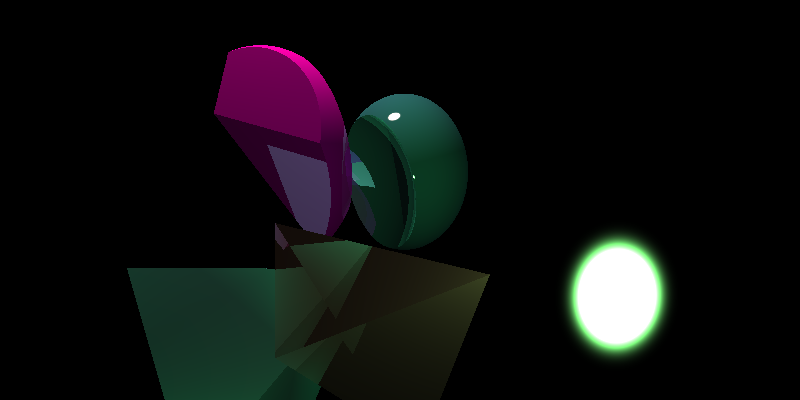
\includegraphics[width=\textwidth]{../img/pic.png}
		\caption{Example picture}
		\label{f:pic}
	\end{figure}